\chapter{Die Quelle der Daten}
Die Daten werden aus einer Webseite \cite{Daten} extrahiert. Diese Webseite wird kontinuierlich aktualisiert. Dabei ist der Inhalt h\"ochst dynamisch dargestellt. Beispielsweise wird nur der Inhalt einer Tabelle bei einem Klick aktualisiert.\\
Dadurch kann ein einfaches Parsen der Webseite nicht stattfinden.
Hierzu werde ich eine M\"oglichkeit beschrieben, was den Inhalt trotz des Hindernisses laden kann.
\\
Der Urheber der Webseite ("FlashScore") hat unter anderem viele weitere Seiten eingestellt. 
Alle haben die selbige Struktur und k\"onnen so, durch Anpassen der Links auf die neue Seite, ebenfalls bearbeitet werden.\\
\\
Deshalb muss man sich beim Ausw\"ahlen der Quelle f\"ur die Daten nicht nur auf Eishockey beschr\"anken, sondern kann auch seinen Lieblingssport aussuchen.


\chapter{PhantomJS}
PhantomJS \cite{Webkit} ist ein WebKit, welches mittels einer JavaScript API gesteuert wird und so jeden Webbrowser simulieren kann.\\
Dadurch kann man auf den Quelltext der Webseite zugreifen, wie in einem richtigen Browser.
Jedoch ist es nur die reine API f\"ur die Simulation des Browsers. 
Darauf aufbauend existieren viele Frameworks.
Unter anderem das Framework bzw. Test-Framework CasperJS.
Dieses wird sp\"ater noch weiter erl\"autert.

Die wichtigsten Merkmale von PhantomJS:
\begin{itemize}
\item Auswahl des zu simulierenden Browsers
\item Laden von Bildern der Webseite
\item Skripte, die zum Parsen der Seite verwendet werden
\end{itemize}
\newpage

\chapter{CasperJS}
CasperJS \cite{CasperJS} ist ein Framework welches auf PhantomJS \cite{Webkit} aufbaut.
Es bietet viele Funktionen um auf der Seite zu navigieren und alle Funktionen zu nutzen, die auch ein \"ublicher Nutzer einer Webseite nutzen k\"onnte.
Hierzu einige wichtige Merkmale:
\begin{itemize}
\item Navigieren innerhalb der Webseite
\item Folgen von Links
\item Erstellen von Screenshots 
\item Durchlaufen des DOM der Webseite
\item Erstellung von eigenen Tests auf der Webseite
\end{itemize}
F\"ur mein Projekt verwende ich nur einen Bruchteil der Funktionalit\"at von CasperJS. Denn mit Hilfe von CasperJS kann noch viel mehr auf einer Webseite ausgef\"uhrt werden.
Zum Beispiel kann ein Laufzeittest durchgef\"uhrt oder auch ein einfaches Ausf\"ullen eines Formulars simuliert werden.\\
\\
Weitere Anwendungsbeispiele sind hierzu auf den jeweiligen Seiten von CasperJS \cite{CasperJS} und PhantomJS\cite{Webkit} zu finden.
\newpage
Beispiel zum Einstieg in ein CasperJS-Skript:
\begin{lstlisting}
var casper = require('casper').create({
  verbose: true,
  logLevel: 'error',
  pageSettings: {
    loadImages: false,
    loadPlugins: false,
    userAgent: 'Mozilla/5.0 (Windows NT 6.2; WOW64) AppleWebKit/537.36 
    			(KHTML, like Gecko) Chrome/29.0.1547.2 Safari/537.36'
  },
  clientScripts: ['/Users/Arti/Downloads/jquery-2.1.1.js']
});
\end{lstlisting}


\chapter{Generierung der Daten}
Das Script zum Extrahieren der Daten dieser Webseite \cite{Daten} f\"angt immer auf der Startseite der jeweiligen Liga an.
Daraufhin folgt es allen Links, die noch in dieser Liga spielen, also den Unterligen.\\
\\
Dadurch das in jedem Land mindestens eine Liga vorhanden ist, gibt es diverse Startpunkte f\"ur das Skript.
Um dies zu erleichtern, gibt es noch ein weiteres Skript, welches f\"ur jede Liga, die auf der Seite existiert, das eigentliche Skript aufruft und die generierten Daten auf eine Datei im selben Verzeichnis umleitet.\\
\begin{lstlisting}
#!/bin/bash
casperjs $1 --site=http://www.ergebnisselive.com/eishockey/deutschland/del/ 
			> tableDel.xml
echo "</table></section></article>" >> tableDel.xml
casperjs $1 --site=http://www.ergebnisselive.de/eishockey/finnland/liiga/ 
			> tableLiiga.xml
echo "</table></section></article>" >> tableLiiga.xml
casperjs $1 --site=http://www.ergebnisselive.de/eishockey/osterreich/ebel/ 
			> tableEbel.xml
echo "</table></section></article>" >> tableEbel.xml
casperjs $1 --site=http://www.ergebnisselive.de/eishockey/russland/khl/ 
			> tableKhl.xml
echo "</table></section></article>" >> tableKhl.xml
casperjs $1 --site=http://www.ergebnisselive.de/eishockey/schweden/elitserien/ 
			> tableElitserien.xml
echo "</table></section></article>" >> tableElitserien.xml
casperjs $1 --site=http://www.ergebnisselive.de/eishockey/schweiz/nla/ 
			> tableNla.xml
echo "</table></section></article>" >> tableNla.xml
casperjs $1 --site=http://www.ergebnisselive.de/eishockey/tschechien/extraliga/ 
			> tableExtraliga.xml
echo "</table></section></article>" >> tableExtraliga.xml
casperjs $1 --site=http://www.ergebnisselive.de/eishockey/usa/nhl/ 
			> tableNhl.xml
echo "</table></section></article>" >> tableNhl.xml
\end{lstlisting}

Als Parameter bekommt dieses Skript lediglich den Pfad zum CasperJS Skript, welches im Skript den Parameter \$1 im obigen Skript ersetzt. \\

Da das CasperJS - Skript sehr umfangreich ist, wird dieses im Github \cite{Code} abgelegt und liegt auch diesem Dokument bei.


\chapter{Generierung aus Docbook}
Die Generierung kann mit jeder beliebigen Software wie z.B. OxyGen o.\"a. erfolgen.
In meinem Beispiel benutze ich das Dep4E-Plugin f\"ur Eclipse.
Dadurch kann ein Projekt erzeugt werden, welches dann per XML-File konfiguriert werden kann und mit Hilfe von ANT das Docbook-XML in das gew\"unschte Format formatiert.\\
Alle Dateien, die vom CasperJS generiert werden, m\"ussen in das Projekt kopiert werden.
Hierzu ist in der Abbildung 'Dep4E Plugin'  ein \"Uberblick zu einem solchen Projekt im Eclipse.
\begin{figure}[h!]
  \caption{Dep4E Plugin}
  \centering
    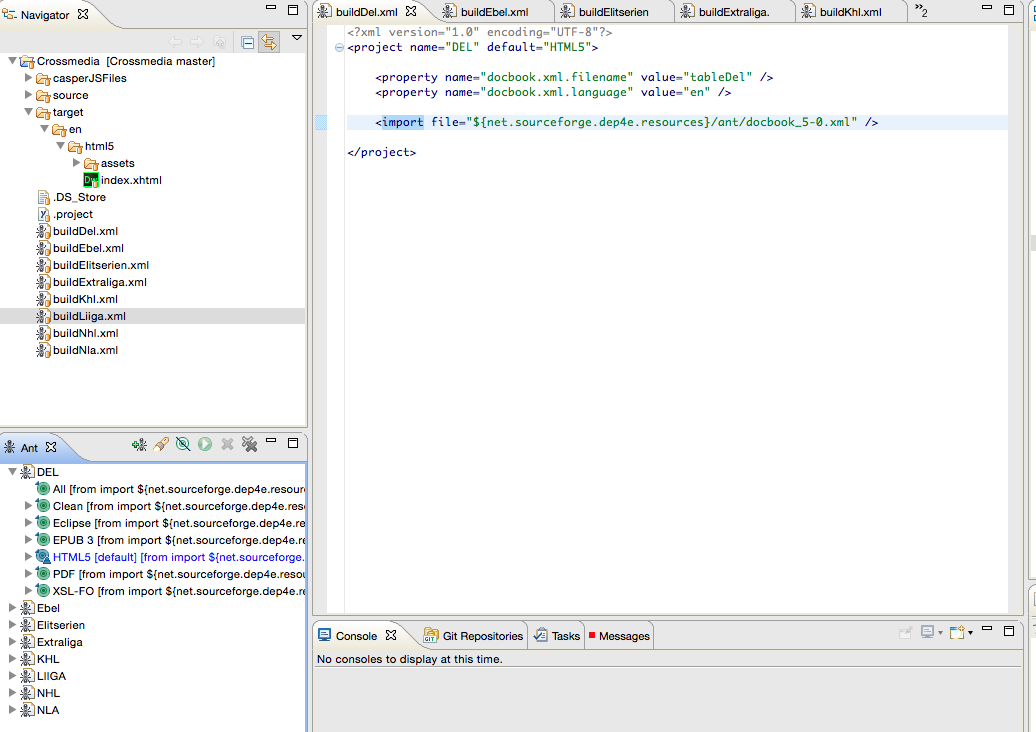
\includegraphics[scale=0.39]{Abbildungen/Dep4Plugin}
\end{figure}

\chapter{Zusammenfassung}
Insgesamt konnte ich die Extraktion zwar leider nicht komplett generisch gestalten. Jedoch kann das Skript auch auf jeder beliebigen Seite, die von FlashScore eingestellt ist, benutzt werden.
Auch kann auf das Archiv zugegriffen werden, da daf\"ur nur Link zur Webseite angepasst werden muss.
Aus den extrahierten Daten kann auch im Weiteren ein Diagramm erzeugt werden, da sich doch rausstellte, dass in Tschechien, Russland der den USA doch wesentlich mehr Mannschaften spielen als in Deutschland oder anderen L\"andern.
Da aber die Daten bereits vorliegen ist das dann keine grosse H\"urde mehr.
Fast alles konnte automatisiert werden, bis auf das Kopieren der generierten Daten in das Eclipse-Projekt. 
Durch die Benutzung eines anderen Programmes kann dies aber auch automatisiert werden.\\
\\
Das Vorgehen kann auch auf beliebige Seiten von FlashScore angewendet werden, da das Theme von deren Seiten \"ahnlich ist.
Somit kann jeder seine Liebllingsseite und auch seinen gew\"unschten Sport aussuchen.\\
\\
Da aus der erzeugten Tabelle ebenfalls ein Diagramm erzeugt werden k\"onnte, kann dieses dann z.B. auch in einer eigenen Seite als interessantes Widget oder \"ahnliches eingebunden werden oder auch direkt in Fachzeitschriften, wenn sich diese z.B. auf die Vorjahre einer Mannschaft beziehen.\\
\\
Das Verfahren und auch das Skript ist also, mit kleineren Anpassungen, in verschiedensten Richtungen einsetzbar und ebenfalls in verschiedenen Medien.

